 %%%%%%%%%%%%%%Empieza la presentacion%%%%%%%%%%%%%%%%%%%%%%%%%%%%%%%%%%%%

%\begin{frame}
%\frametitle{Esquema}
 %   \tableofcontents
%\end{frame}

\subsection{Una variable aleatoria}

\begin{frame}\frametitle{Definición de una variable aleatoria}
  \begin{itemize}
    \item \alert{Variable aleatoria$^1$ $X$ (continua o discreta)}:
    \begin{itemize}
      \item Representa el resultado de un experimento aleatorio.
      \item Su valor no es conocido a priori.
      \item ¿Cómo podemos caracterizarla?
      \begin{itemize}
        \item ¿Que valores puede tomar?
        \item ¿Es igual de probable cada valor?
      \end{itemize}
    \end{itemize}
  \end{itemize}

  \begin{columns}[T]
    \begin{column}{5cm}
      \scriptsize
      \centering \color{olivegreen} Ejemplo discreto: X valores de un dado
      \color{gray}$p_X(x)=\frac{1}{6}$

      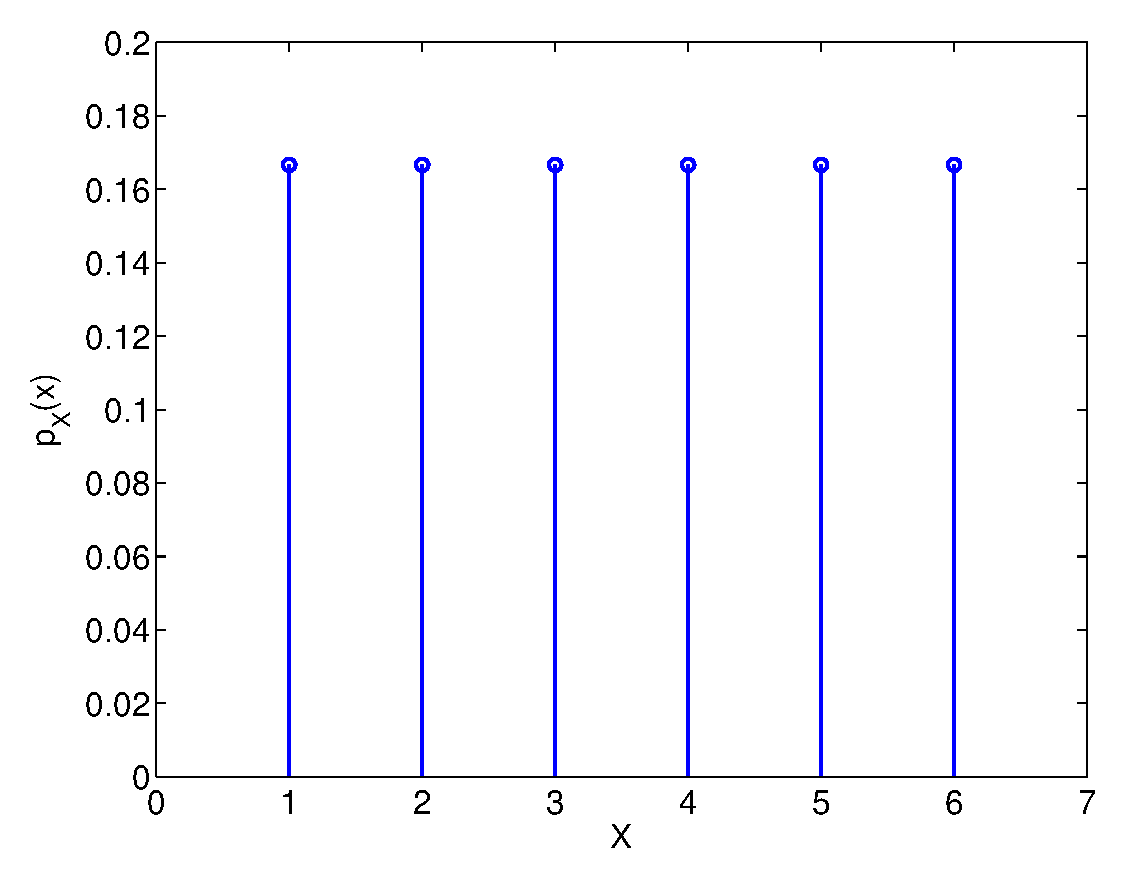
\includegraphics[width=3cm]{./Figures/ProbDiscreta.eps}
    \end{column}
    \begin{column}{6cm}\centering
      \scriptsize

      \centering \color{olivegreen} Ejemplo continuo: X tiempo de espera

      \color{gray}$p_X(x)=\mathcal{U}_{X\in[0,30]}(x)$

      \vspace{0.2cm}
      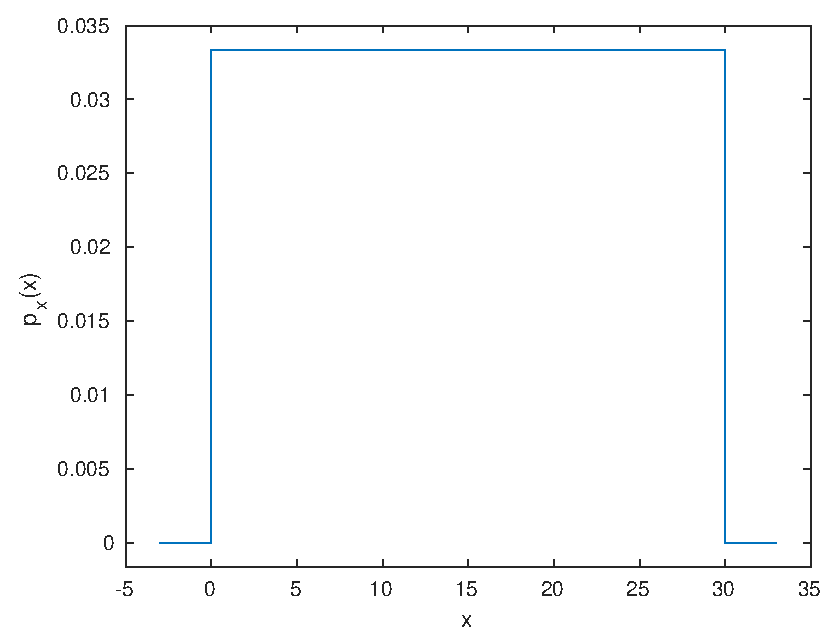
\includegraphics[height=2cm]{./Figures/ProbContinua.eps}
      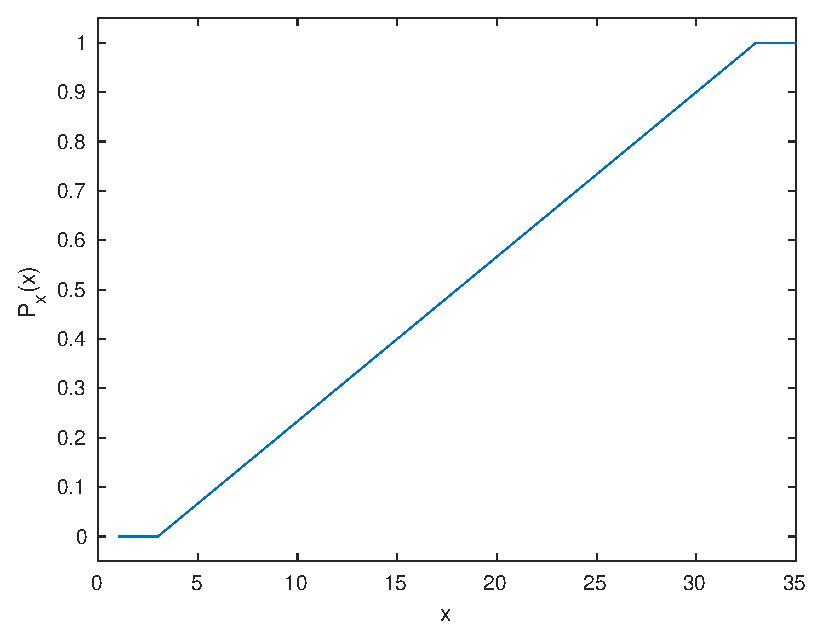
\includegraphics[height=2cm]{./Figures/ProbDistContinua.eps}
    \end{column}
  \end{columns}


  \rule{10cm}{0.04ex}

  \scriptsize
  $^1$En estadística es habitual definir la variable aleatoria con mayúsculas y sus valores con minúsculas.
\end{frame}



\begin{frame}\frametitle{Definición de una variable aleatoria}
  \begin{itemize}
    \item \alert{Para variables discretas:}
    \vspace{0.1cm}
    \begin{itemize}\footnotesize
      \item Función de \color{olivegreen}\emph{masa de probabilidad}: \color{blue}$p_X(x_i)=Probabilidad(X=x_i)$\color{black}
      \vspace{0.1cm}
      \item Propiedades:
      \begin{itemize}
        \item $0\le p_X(x_i)\le 1$
        \vspace{0.1cm}
        \item $\sum_{x\in X} p_X(x)=1$
      \end{itemize}
    \end{itemize}
    \vspace{0.2cm}
    \item \alert{Para variables continuas:}
    \vspace{0.1cm}
    \begin{itemize}\footnotesize
      \item \color{olivegreen}\emph{Distribución de probabilidad}: \color{blue}$P_X(x)=Probabilidad(X\le x)$\color{black}
      \vspace{0.1cm}
      \item \color{olivegreen}\emph{Densidad de probabilidad}: \color{blue}$p_X(x)=\frac{\partial P_X(x)}{\partial x}$\color{black}
      \vspace{0.1cm}
      \item Propiedades:
      \begin{itemize}
        \item $p_X(x)\ge 0$ $\rightarrow P_X(x)$ es una función creciente
        \vspace{0.1cm}
        \item $P_X(x)=\int_{-\infty}^x p_X(y)dy \rightarrow P_X(\infty)=1$
      \end{itemize}
    \end{itemize}
  \end{itemize}



  % \rule{10cm}{0.04ex}

  % \scriptsize
  % $^1$En estadística es habitual definir la variable aleatoria con mayúsculas y sus valores con minúsculas.
\end{frame}

%%%%%%%%%%%%%%


\begin{frame}\frametitle{Estadísticos}
  % \begin{itemize}
  %   \item ¿Qué más podemos decir sobre la variable aleatoria?
    \begin{itemize}
      \item Un \alert{estadístico} es una medida cuantitiva de una muestra.
      \begin{itemize}
        \item Valor esperado de alguna función $g(x)$.
        \begin{itemize}
          \vspace{0.1cm}
          \item \alert{Continuo:} \hspace{0.1cm}\\\vspace{0.1cm}$E(g(X))=\int_{-\infty}^{\infty}g(x) p_X(x)dx$
          \vspace{0.1cm}
          \item \alert{Discreto:}\\\vspace{0.1cm}$E(g(X))=\sum_{x_i \in X} g(x_i)p_X(x_i)$
        \end{itemize}
      \item Respecto a la probabilidad $p_X(x)$.
      \end{itemize}
      \item Trata de inferir o estimar una propiedad de la población.
    \end{itemize}
    \footnotesize
        % \item Estadísticos frecuentes:
    % \begin{itemize}
    %   \item $\mu_x=E\{X\}$ (media)
    %   \item $\sigma_x^2=E\{(X-\mu_x)^2\}$ (varianza)
    %   \item $E\{X^2\}=\sigma_x^2+\mu_x^2$ (valor cuadrático medio)
    % \end{itemize}
  % \end{itemize}
\end{frame}
  

\begin{frame}\frametitle{Estadísticos de una variable aleatoria}
  \footnotesize

% \vspace{-0.2cm}
  \begin{itemize}
    \item Estadísticos/características habituales (expresiones continuas$^1$)

    \begin{itemize}\footnotesize
      \item \alert{Valor medio}:\\\vspace{0.1cm}$\mu_X \triangleq E(X)$ $=\int_{-\infty}^{\infty}x p_X(x)dx$
      \item \alert{Valor cuadrático medio:}\\\vspace{0.1cm}$E(X^2)$ $=\int_{-\infty}^{\infty}x^2 p_X(x)dx$
      \item \alert{Varianza$^2$:}\\\vspace{0.1cm}$\sigma^2_X \triangleq E((X-\mu_x)(X-\mu_x))=\int_{-\infty}^{\infty}(x-\mu_x)(x-\mu_x) p_X(x)dx$ $=E(X^2)-\mu_x^2$
    \end{itemize}

  \end{itemize}

% \vspace{-0.3cm}

  \rule{11cm}{0.04ex}
  \scriptsize
  $^1$La relación discreta se puede sacar de la continua, construyendo una función densidad de probabilidad para la variable aleatoria discreta:  $p_{X_C}(x)=\sum_{x_i \in X} p_X(x_i)\delta(x-x_i) \rightarrow$
  $E(g(X_C))\!=\!\int_{-\infty}^{\infty}\!g(x)\! \sum_{x_i \in X} p_X(x_i)\delta(x\!-\!x_i)dx\!=\!\sum_{x_i \in X} g(x_i)p_X(x_i)=E(g(X))$. Equivale a sustituir las integrales por sumarios en las relaciones de las variables continuas. Por lo tanto, podemos definir únicamente las relaciones continuas y extrapolar las discretas.

  \vspace{0.2cm}

  $^2$Relación entre $\sigma^2_X$, $\mu_X$ y $E(X^2)$:  $\sigma^2_X\!=\!\! \int_{-\infty}^{\infty}\!\!(x^2\!-\!2 \mu_X x\!+\! \mu_X^2) p_X(x)dx=$ $=E(X^2)-2\mu_X \int_{-\infty}^{\infty}x p_X(x)dx+ \mu_X^2  \int_{-\infty}^{\infty}p_X(x)dx=E(X^2)-2\mu_X^2+\mu_X^2 $

\end{frame}

%%%%%%%%%%%%%%%%%%%%%%%%%%%%%%%%%%%%%%%%%%%%%%%%%


\begin{frame}\frametitle{Variables aleatorias comunes}
  \begin{itemize}
    \item \alert{Distribución uniforme}:\hspace{0.2cm}
    \small$p_X(x)=\mathcal{U}_{X \in [a,b]}(x)=\left \{\begin{array}{cl}\frac{1}{b-a}  &  x\in [a,b] \\0 &c.c.\end{array} \right .$
    \begin{itemize}
      \footnotesize
        \vspace{0.1cm}
        \item \color{blue}$\mu_x=\int_{-\infty}^{\infty}x p_X(x)dx=\frac{b+a}{2}$\color{black}\\
        \hspace{0.5cm}\color{cyan}$\int_a^b\frac{x}{b-a} dx=\frac{x^2}{2(b-a)}|_a^b=\frac{b^2-a^2}{2(b-a)}=\frac{b+a}{2}$\color{black}
        \vspace{0.1cm}
        \item \color{blue}$E(X^2)=\int_{-\infty}^{\infty}x^2 p_X(x)dx=\frac{b^2+a^2+ab}{3}$\color{black}\\
        \hspace{0.5cm}\color{cyan}$\int_a^b\frac{x^2}{b-a} dx=\frac{x^3}{3(b-a)}|_a^b=\frac{b^3-a^3}{3(b-a)}=\frac{b^2+a^2+ab}{3}$\color{black}
        \vspace{0.1cm}
        \item \color{blue}$\sigma^2_X=E(X^2)-\mu^2_X=\frac{(b-a)^2}{12}$\color{black}
      \end{itemize}
    \end{itemize}
    \centering
    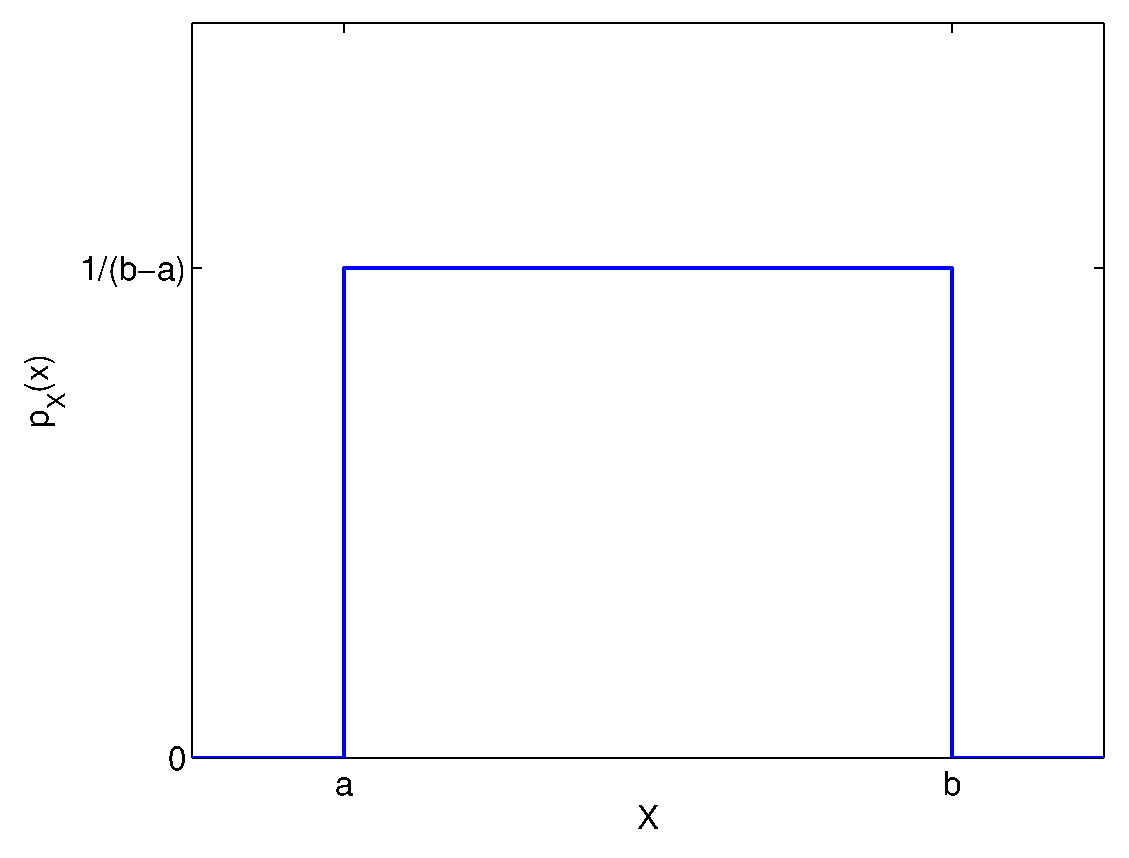
\includegraphics[width=3.5cm]{./Figures/ProbUniforme.eps}
\end{frame}


\begin{frame}\frametitle{Variables aleatorias comunes}
  \begin{itemize}
    \item \alert{Distribución gaussiana}:\hspace{0.2cm}
    \small$p_X(x)=\mathcal{N}_{X}(x;\mu,\sigma)=\frac{1}{\sqrt{2\pi \sigma^2}} e^{-\frac{(x-\mu)^2}{2\sigma^2}}$
    \begin{itemize}
      \footnotesize
      \item \color{blue}$\mu_x=\int_{-\infty}^{\infty}x p_X(x)dx=\mu$\color{black}
      \vspace{0.1cm}
      \item \color{blue}$E(X^2)=\int_{-\infty}^{\infty}x^2 p_X(x)dx=\sigma^2+\mu_x^2$\color{black}
      \vspace{0.1cm}
      \item \color{blue}$\sigma^2_X=E(X^2)-\mu^2_X=\sigma^2$\color{black}
      \vspace{0.1cm}
    \end{itemize}
  \end{itemize}
  \centering
  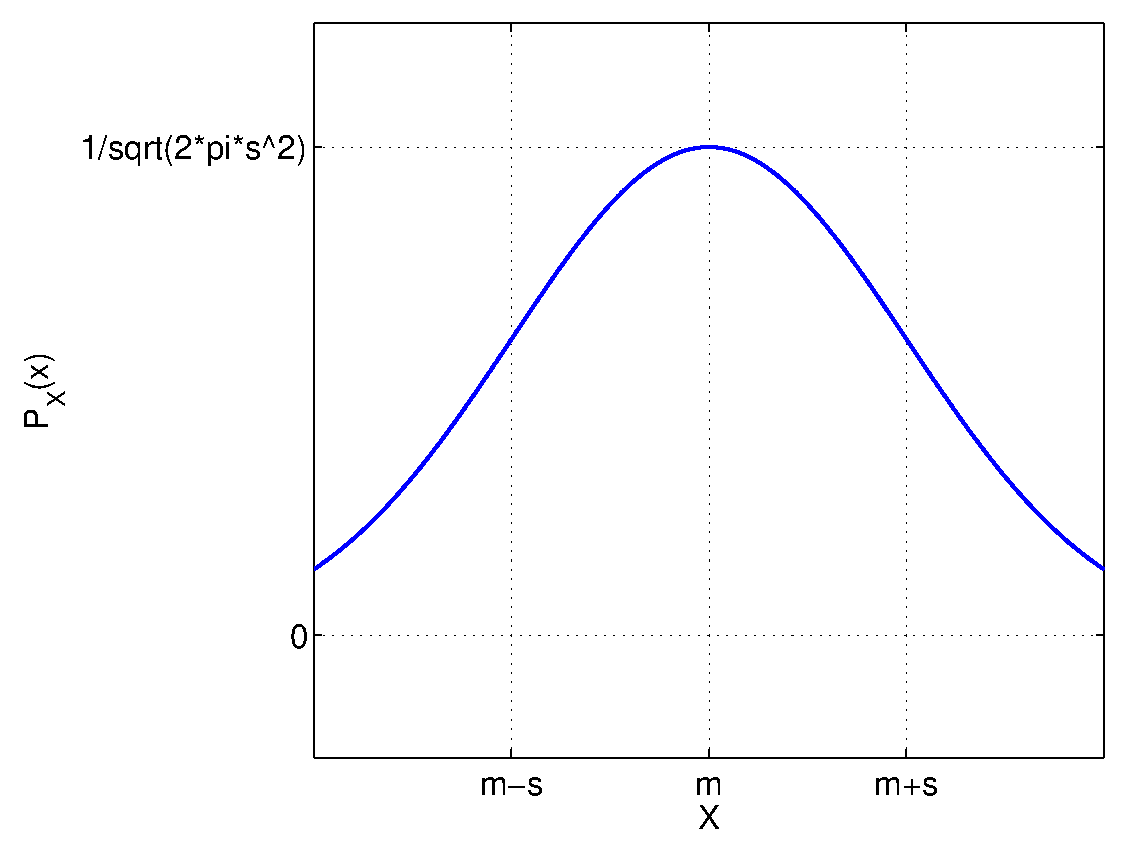
\includegraphics[width=3.5cm]{./Figures/ProbGauss.eps}
\end{frame}
    



\begin{frame}
\frametitle{Muestreo de una variable aleatoria I}

\footnotesize

\begin{itemize}
  \item \alert{Muestreo de una variable aleatoria:}
  \begin{itemize}\scriptsize
    \item Obtener sus valores (muestras) de acuerdo con la densidad de probabilidad.
    \item Matemáticamente representaremos la función como: \color{olivegreen}$x \sim p_X(x)$\color{black}
  \end{itemize}  
  \item \alert{¿Cómo generar las muestras?}
  \begin{itemize}\scriptsize
    \item  Experimentalmente, excitando/observando la respuesta 
    \begin{itemize}\scriptsize
      \item de un proceso aleatorio 
      \item de un proceso determinista con una entrada aleatoria
    \end{itemize}
    \item Utilizando un generador de números pseudo-aleatorios:

    \begin{itemize}\scriptsize
      \item Probabilidad \alert{discreta}: \color{blue}$p_x(x_i)$ con $i\in [1:N]$\color{black}\\\scriptsize
      \color{blue}$\bullet\:\:$\color{black} Equiprobables con Matlab: \color{blue}\texttt{randi($\#_{valores}$,filas,col)}\color{black}\\
      \color{blue}$\bullet\:\:$\color{black} No equiprobables: método de la ruleta
      \item Probabilidad \alert{uniforme}: \color{blue}$\mathcal{U}_{X\in [a,b]}(x)$\color{black}\\\scriptsize
      \color{blue}$\bullet\:\:$\color{black} Matlab: \color{blue}\texttt{a+(b-a)*rand(filas,col)}\color{black}\\
      \color{blue}$\bullet\:\:$\color{black} Secuencias básicas: $x_{i+1}=(a*x_i+c)\mod m$.
      \hspace{3.2cm}\color{gray}{Ejemplo con $a=65539, m=2^{29}$}\color{black}
      \item Probabilidad \alert{gaussiana}: \color{blue}$\mathcal{N}_{X}(x;\mu,\sigma)$\color{black}\\\scriptsize
      \color{blue}$\bullet\:\:$\color{black} Matlab: \color{blue}\texttt{$\mu$+$\sigma$*randn(filas,col)}\color{black}\\
      \color{blue}$\bullet\:\:$\color{black} Transformada de Box-Muller (a partir de la uniforme)
      \item Probabilidades \alert{genéricas}:\\\scriptsize
      \color{blue}$\bullet\:\:$\color{black}Muestreo por rechazo, por importancia\\
      \color{blue}$\bullet\:\:$\color{black} Muestreo de mezclas
    \end{itemize}
    \end{itemize}
  \end{itemize}
\end{frame}

\begin{frame}
\frametitle{Muestreo de una variable aleatoria II}

\footnotesize


\begin{columns}[T]
\begin{column}{7cm}
\begin{itemize}
\item \alert{Método de la ruleta:}
\begin{itemize}
\footnotesize
\item $p(x_i)$
\item Muestreo variable auxiliar:
$y \sim \mathcal{U}_{y\in [0,1]}(y)$
\item $x=\{ j |\sum_{i=1}^{j-1}p(x_i) < y<\sum_{i=1}^j p(x_i)\}$
\end{itemize}
 \end{itemize}
\end{column}
\begin{column}{4cm}
\visible<2->{
\lstinputlisting{./Matlab/Ruleta.m}
}
\end{column}
\end{columns}

\vspace{-0.2cm}

\visible<3->{

\begin{columns}[T]
\begin{column}{7cm}
\begin{itemize}
\item \alert{Transformada de Box-Muller:}
\begin{itemize}
\footnotesize
\item  $\mathcal{N}(x,\mu\!=\!0,\sigma^2\!=\!1)$
\item Muestreo de 2 variables auxiliares:

\hspace{0.3cm}$y_1 \sim \mathcal{U}_{y\in [0,1]}(y)$

\hspace{0.3cm}$y_2 \sim \mathcal{U}_{y\in [0,1]}(y)$
\item Transformación de las muestras:

\hspace{0.3cm}$r=\sqrt{-2\log(y_1)}$

\hspace{0.3cm}$\theta=2\pi y_2$

\hspace{0.3cm}$x_1=r \cos(\theta)$

\hspace{0.3cm}$x_2=r \sin(\theta)$

\scriptsize
Se genera un par, para hacer una guassiana de dos dimensiones o un complejo. Se puede usar solo uno.
\end{itemize}
 \end{itemize}

\end{column}
\begin{column}{4cm}
\visible<4->{
\lstinputlisting{./Matlab/BoxMuller.m}}
\end{column}
\end{columns}

}


 \end{frame}

%%%%%%%%%%%%%%%%%%%%%%%%%%%%%%%%%%%%%%%%%%%%%%%%



\begin{frame}
\frametitle{Muestreo de una variable aleatoria III}

\footnotesize


\begin{columns}[T]
\hspace{-0.5cm}\begin{column}{7cm}
\begin{itemize}
\item \alert{Método de muestreo por rechazo:}
\begin{itemize}
\footnotesize
\item Función de probabilidad genérica $p(x)$
\item Las muestras se obtienen de una $q(x)$ auxiliar que debe cumplir que para algún M que Mq(x)-p(x)>0.  Este hecho fuerza a que tengan el mismo soporte (que $q(x)\ne 0$ sobre los mismos puntos x que $p(x)\ne 0$).
\item Las $x\sim q(x)$ son también muestras de $p(x)$ si se cumple que $yMq(x)<p(x)$ con $y \sim \mathcal{U}_{y\in [0,1]}(y)$
\end{itemize}
 \end{itemize}


 \hspace{2cm}\includegraphics[width=3.5cm]{./Figures/MuestreoRechazo.eps}

\end{column}
\begin{column}{4,5cm}

\visible<2->{

\lstinputlisting{./Matlab/MuestreoRechazo.m}}
\end{column}
\end{columns}

\vspace{-0.2cm}



 \end{frame}


%%%%%%%%%%%%


\begin{frame}
\frametitle{Muestreo de una variable aleatoria IV}

\footnotesize


\begin{columns}[T]
\begin{column}{6.8cm}
\begin{itemize}
\item \alert{Muestreo de una mezcla:}
\begin{itemize}
\footnotesize
\item Función de probabilidad genérica $p(x)=\sum_{i=1}^La_ip_i(x)$, con $\sum_{i=1}^L a_i=1$
\item Para muestrearla, podemos seguir el siguiente proceso:
\begin{itemize}
\item Elegimos la componente de la mezcla (el valor de la i) utilizando la probabilidad discreta $q(i)=a_i$
\item Muestreamos la x de la componente elegida $x \sim p_i(x)$
\end{itemize}
\end{itemize}
 \end{itemize}

\visible<2->{
 \hspace{2cm}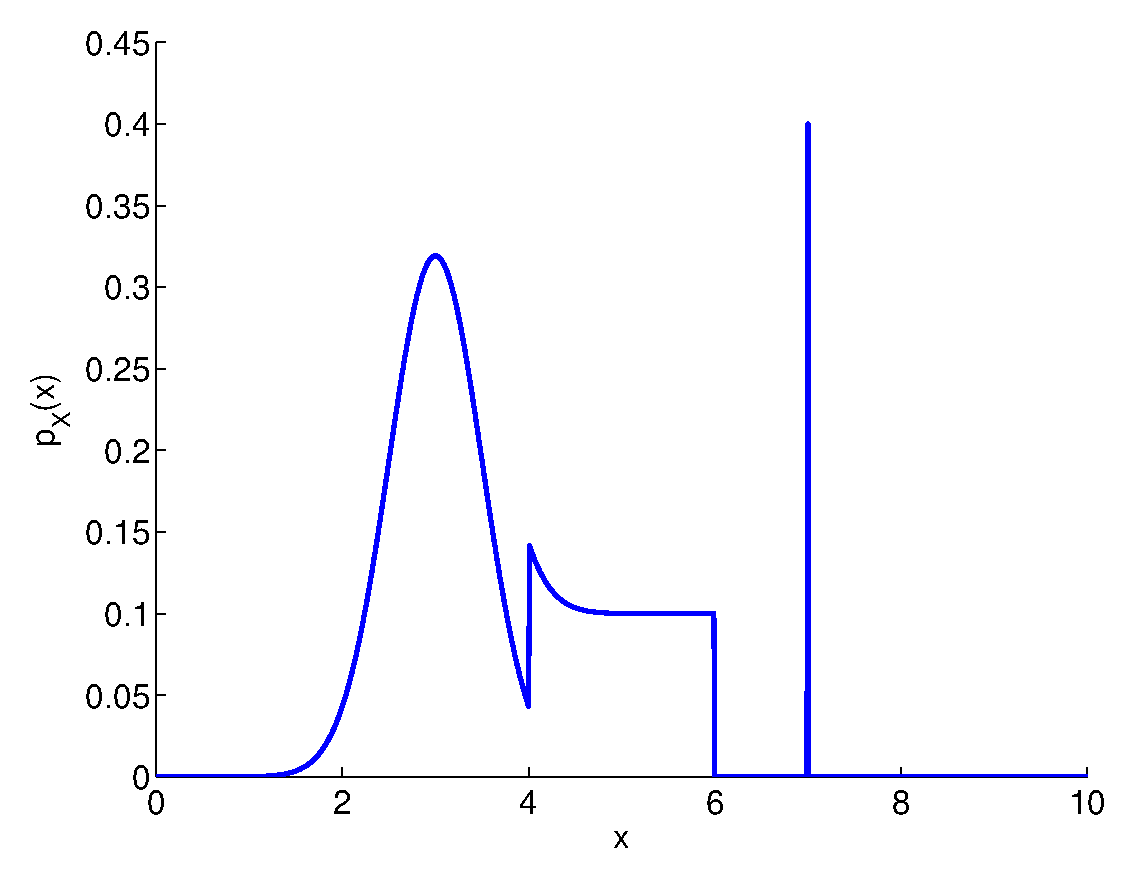
\includegraphics[width=3.5cm]{./Figures/MuestreoMezcla.eps} }

\end{column}
\begin{column}{4.2cm}

\visible<3->{

\lstinputlisting{./Matlab/MuestreoMezcla.m}
}

\visible<2->{
\small
\color{olivegreen}

$p_X(x)=0.4\mathcal{N}(x,3,0.5)+$


\hspace{1.35cm}$0.2\mathcal{U}_{[4,6]}(x)+$

\hspace{1.35cm}$0.4\delta(x-7)$

}
\end{column}
\end{columns}

\vspace{-0.2cm}
 \end{frame}


\begin{frame}
\frametitle{Caracterización de las muestras}

\footnotesize

\vspace{-0.2cm}

\begin{itemize}
\item ¿Que hacer cuando nos proporcionan un conjunto de muestras sin su función de probabilidad?

\visible<2->{

\item El proceso de caracterización de las muestras es conceptualmente análogo al proceso de caracterización de la función de probabilidad. }

\visible<3->{
\item La diferencia reside que en el primer caso no se dispone de una función de probabilidad y en el segundo si.
}

\visible<4->{

\item En el proceso de caracterización de las muestras se puede:
}
\begin{itemize}
\footnotesize

\visible<5->{


\item Intentar estimar la función de probabilidad:
\begin{enumerate}
\item Determinar el tipo de función de probabilidad: histograma de las muestras
\item Determinar los parámetros de la función de probabilidad: a partir de las muestras
\end{enumerate}
}

\visible<6->{

\item Obtener el valor de los estadísticos a partir:
\begin{itemize}
\item De la muestras: Método de Monte-Carlo$^1$
\item De la función de probabilidad que se ha estimado.
}
\end{itemize}
\end{itemize}

\end{itemize}

\vspace{-0.3cm}


\visible<7->{

\rule{11cm}{0.04ex}
\scriptsize

$^1$Los métodos de Monte-Carlo también se utilizan para estimar los estadísticos de funciones de probabilidad conocidas de las que no se pueden calcular las integrales de forma cerrada. El proceso consiste en utilizar los métodos de muestreo para generar muestras de la función de probabilidad y luego el método de Monte-Carlo para estimar el estadístico sobre las muestras generadas.
}
\end{frame}

%%%%%%%%%%%%%%%%%%%%%%%%%%%%%%%%%%%%%%%%%%%%%%

\begin{frame}
\frametitle{Histograma de un conjunto muestral I}

\vspace{-0.3cm}

\footnotesize

\begin{columns}[T]
\hspace{0.2cm}\begin{column}{6cm}
\begin{itemize}
\item El histograma divide el espacio muestral en H segmentos (cubos/bins) continuos de igual tamaño y contabiliza el número de muestras que pertenecen a cada uno de los segmentos.
\end{itemize}
\end{column}
\begin{column}{5cm}
 \hspace{2cm}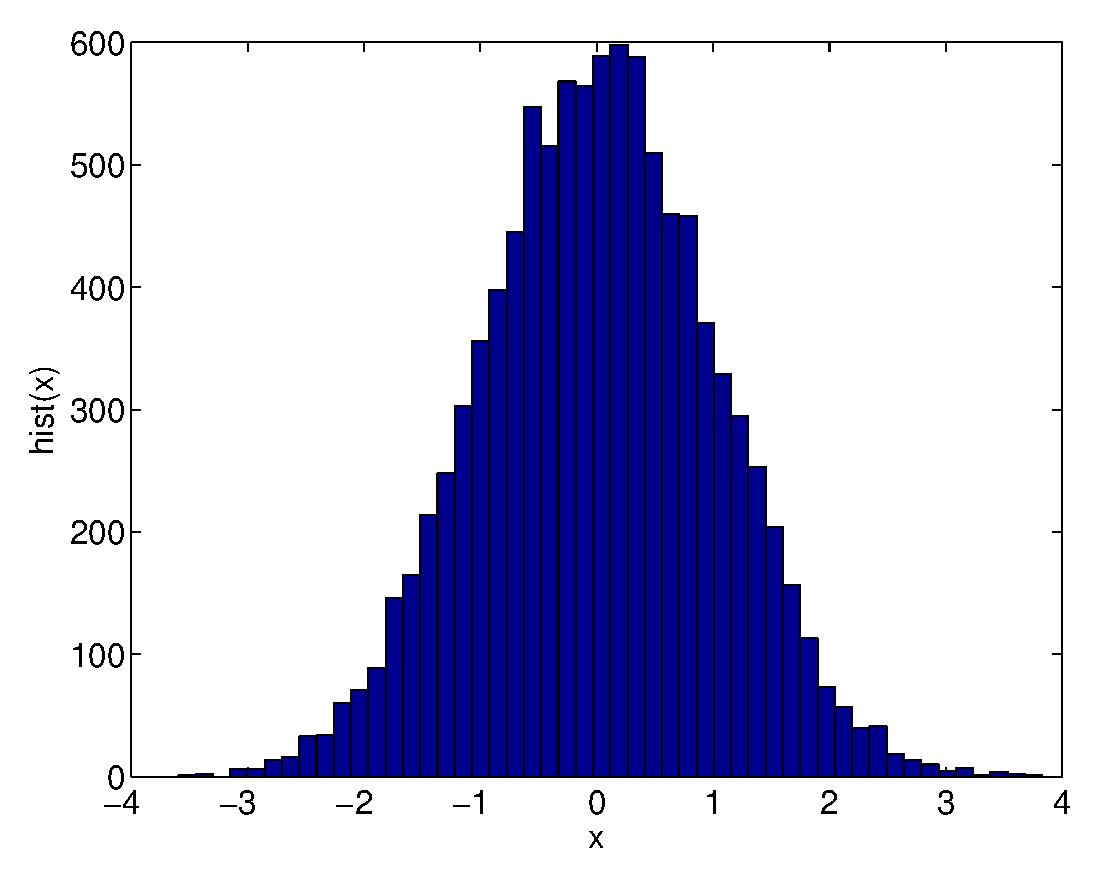
\includegraphics[width=3.1cm]{./Figures/Histograma1.eps}
\end{column}
\end{columns}

\vspace{-0.1cm}

\begin{itemize}

\visible<2->{


\item Podemos utilizarlos para realizar una representación aproximada de la probabilidad de las muestras, siempre y cuando se normalizan las cuentas del histograma de forma que:

\vspace{-0.1cm}

\begin{itemize}
\footnotesize
\item La suma de los valores normalizados del histograma sea 1 para el caso de trabajar con variables aleatorias discretas.
\item El area recogida por el histograma normalizado sea igual a 1 para el caso de trabajar con variables aleatorias continuas.
 \end{itemize}
}
 \vspace{-0.2cm}

\visible<3->{


 \item Una análisis de la forma del histograma (o del histograma normalizado), en la que obviemos los escalones introducidos por la segmentación del espacio muestral, nos puede permitir determinar en algunos casos el tipo de función de probabilidad al que pertenecen las muestras$^1$.

 }
\end{itemize}

\vspace{-0.4cm}


\visible<4->{
\rule{11cm}{0.04ex}
\scriptsize

$^1$En el caso continuo, es conveniente hacer divisiones suficientemente pequeñas para que los escalones no escondan la función de probabilidad real de las muestras.
}
\end{frame}

%%%%%%%%%%%%%%%%%%%%%%%%%%%%%%%%%%%%%%%%


\begin{frame}
\frametitle{Histograma de un conjunto muestral II}
\footnotesize

\begin{columns}[c]
\begin{column}{6.5cm}

\scriptsize

\vspace{-0.2cm}

\color{olivegreen}Ejemplo: Histograma de muestras  $\sim \mathcal{N}_X(x,0,1)$\color{black}

\vspace{-0.2cm}

\lstinputlisting{./Matlab/HistNormal.m}

\end{column}
\begin{column}{4.5cm}
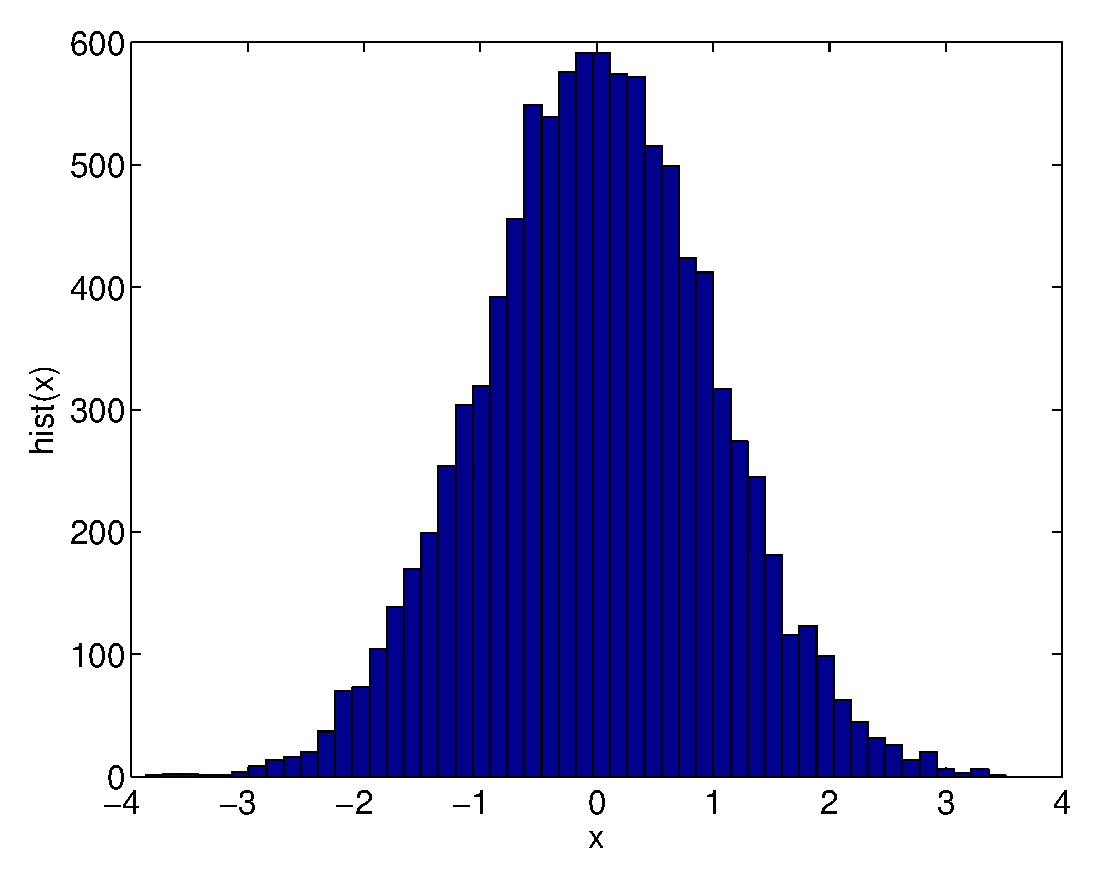
\includegraphics[width=3cm]{./Figures/HistNormal1.eps}

\visible<2->{
\vspace{-1.6cm}
\hspace{1cm}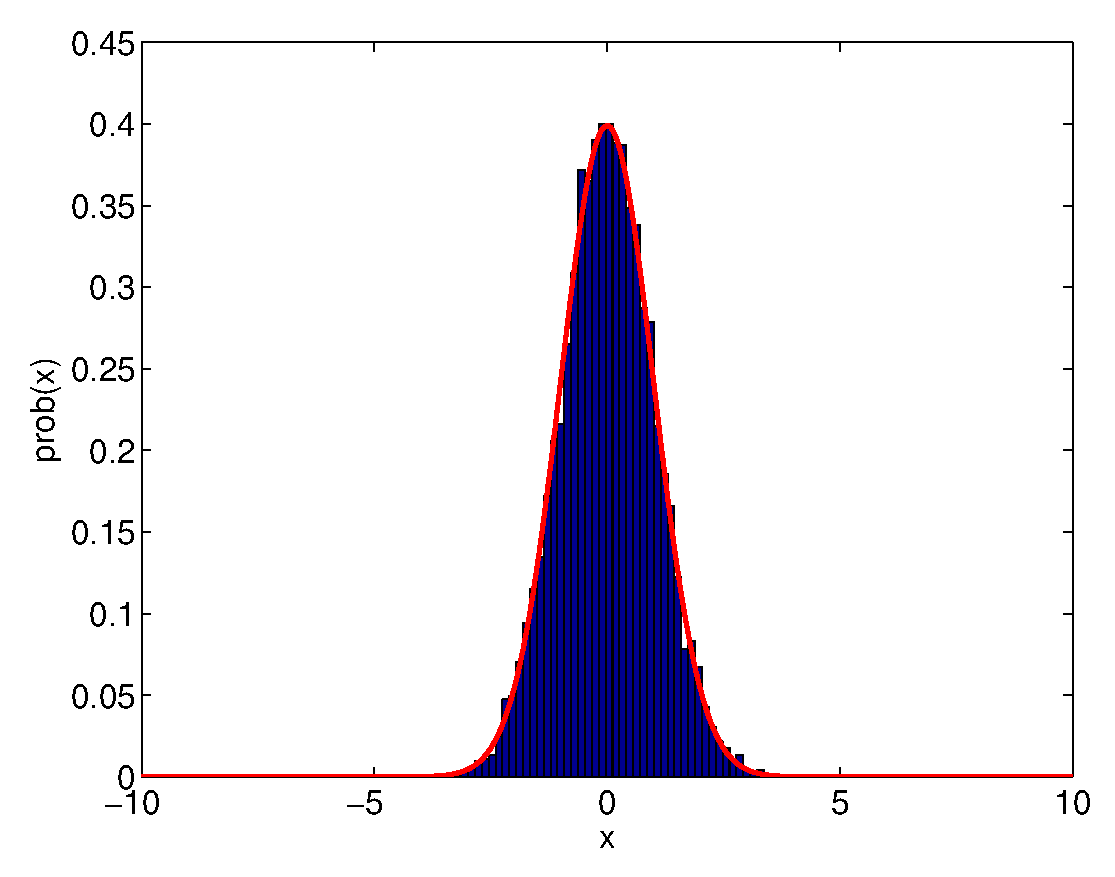
\includegraphics[width=3.5cm]{./Figures/HistNormal2.eps}
}

\end{column}
\end{columns}

% \vspace{0.3cm}

\begin{columns}[c]
\begin{column}{6cm}

\scriptsize
\centering

\visible<3->{

\color{olivegreen}Histograma del ejemplo del rechazo\color{black}

\vspace{0.2cm}

\only<3|handout:0>{\includegraphics[width=4cm]{./Figures/MuestreoRechazo.eps}}\only<4->{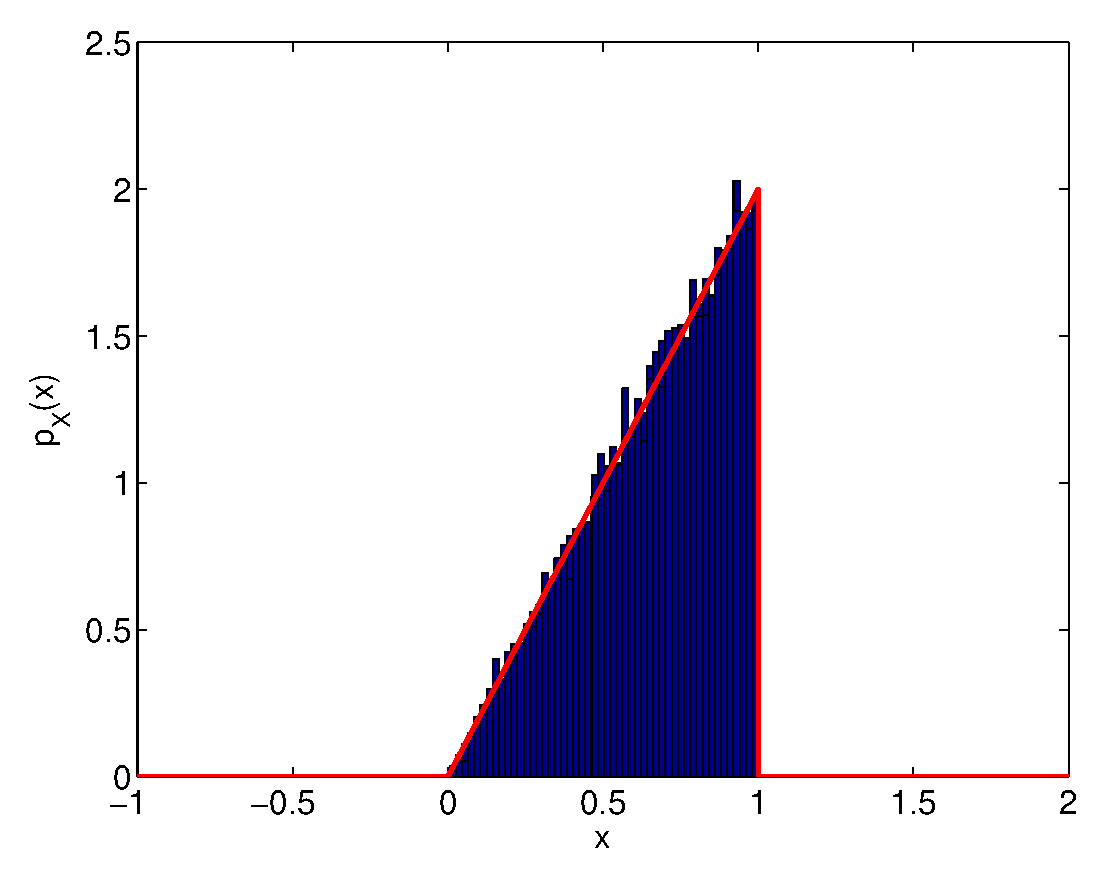
\includegraphics[width=4cm]{./Figures/HistRechazo.eps}}
}



\end{column}
\begin{column}{6cm}
\scriptsize
\centering

\visible<5->{

\color{olivegreen}Histograma del ejemplo de la mezcla\color{black}

\vspace{0.2cm}
\only<5|handout:0>{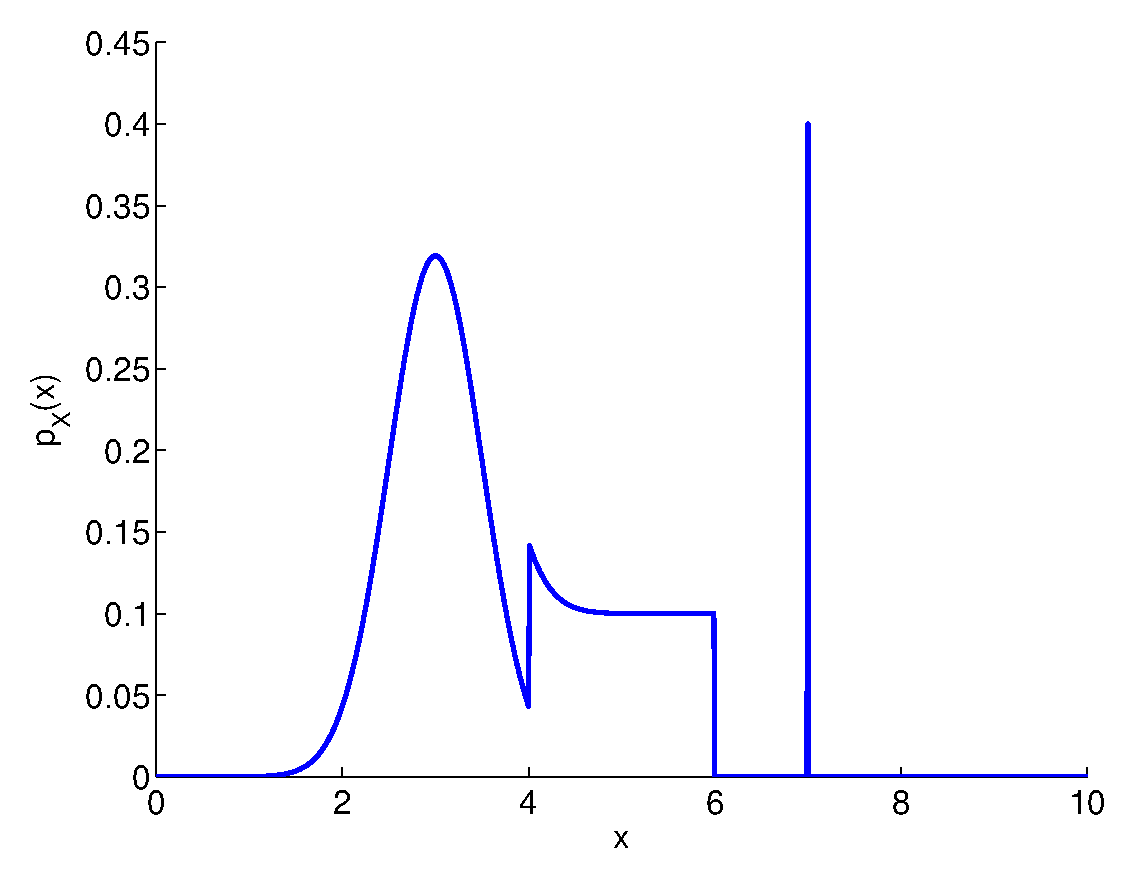
\includegraphics[width=4cm]{./Figures/MuestreoMezcla.eps}}\only<6->{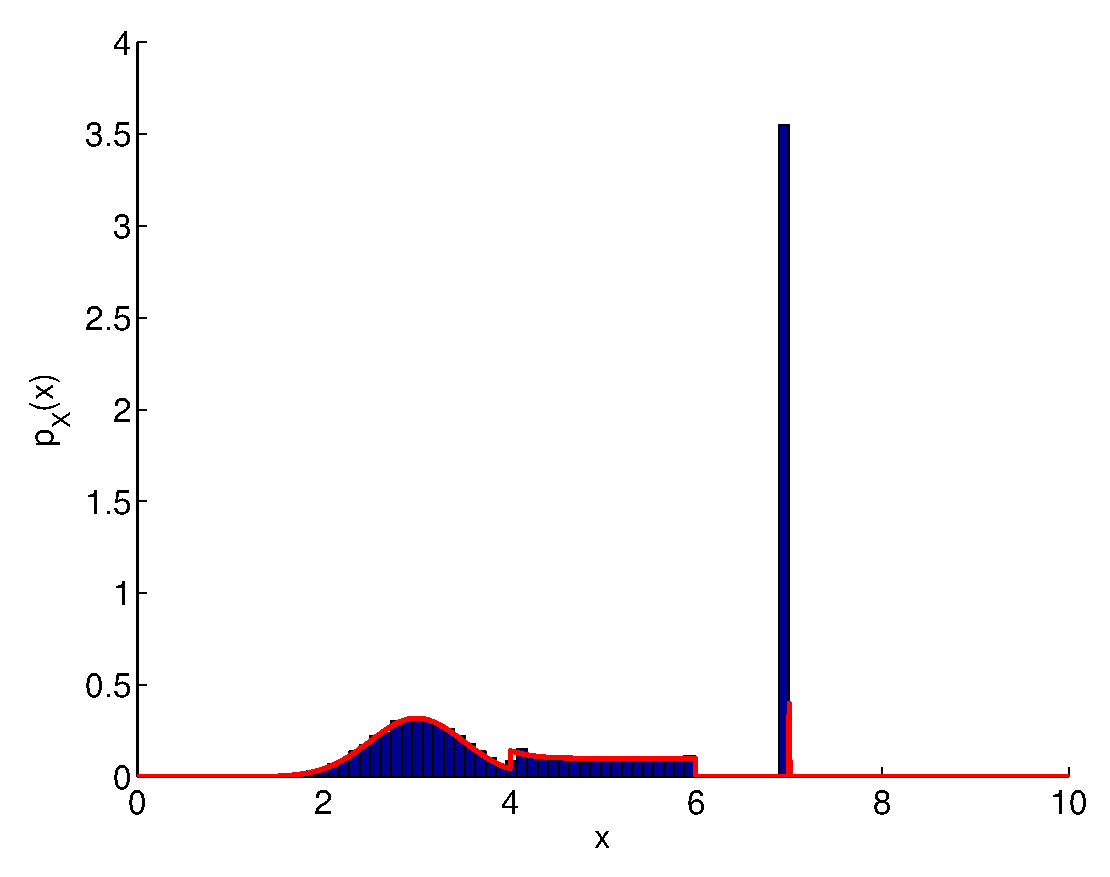
\includegraphics[width=4cm]{./Figures/HistMezcla.eps}}
}

\end{column}
\end{columns}

\end{frame}

%%%%%%%%%%%

\begin{frame}
\frametitle{Métodos de Monte-Carlo}
\footnotesize

\begin{itemize}
\item ¿Como podemos estimar el valor de los estadísticos a partir de las muestras directamente?

\visible<2->{

\item Podemos aproximar  la probabilidad que representan las $N$ muestras por: $p_X(x)=\frac{1}{N}\sum_{n=1}^{N} \delta(x-x_i)$.}

\visible<3->{

\item A partir de esa fórmula, podemos obtener los estadísticos directamente:}
\begin{itemize}
\footnotesize
\visible<3->{

\item  $E(g(X))\!=\!\!\int_{-\infty}^\infty g(x)p_X(x)dx\!=\!\!\int_{-\infty}^\infty g(x) \frac{1}{N}\!\!\sum_{n=1}^{N} \delta(x-x_i) dx\!=$}


\visible<4->{

\vspace{0.1cm}


\hspace{1.15cm}$=\!\frac{1}{N}\sum_{n=1}^{N} \!g(x_i)$

\vspace{0.1cm}


\item Valor medio: $\mu_X=E(X)=\!\frac{1}{N}\sum_{n=1}^{N} \! x_i$

\vspace{0.1cm}


\item Valor cuadrático medio: $E(X^2)=\!\frac{1}{N}\sum_{n=1}^{N} \! x_i^2$

\vspace{0.1cm}


\item Varianza: $\sigma_X^2=E((X-\mu_X)^2)=\!\frac{1}{N}\sum_{n=1}^{N} \! (x_i-\mu_x)^2$
}
\end{itemize}

\visible<5->{

\item Los estadísticos básicos se pueden calcular directamente con Matlab:

\begin{itemize}
\footnotesize
\item Valor medio: \color{blue}\texttt{mu=mean(samples)}\color{black}
\item Varianza$^1$: \color{blue}\texttt{sigma2=var(samples,1)}\color{black}
\item Desviación estandard$^1$ ($\sigma_X$): \color{blue}\texttt{sigma=std(samples,1)}\color{black}
\end{itemize}
}

\end{itemize}

\vspace{-0.2cm}

\visible<5->{


\rule{11cm}{0.04ex}
\scriptsize
$^1$El segundo parámetro tiene que tomar el valor de 1 para que se calcule la varianza dividiendo los resultados entre N.
}

\end{frame}
